\documentclass{beamer}
\usepackage{beamerthemesplit}
\usepackage{wrapfig}
\usetheme{SPbGU}
\usepackage{pdfpages}
\usepackage{amsmath}
\usepackage{cmap} 
\usepackage[T2A]{fontenc} 
\usepackage[utf8]{inputenc}
\usepackage[english,russian]{babel}
\usepackage{indentfirst}
\usepackage{amsmath}
\usepackage{tikz}
\usepackage{multirow}
\usepackage[noend]{algpseudocode}
\usepackage{algorithm}
\usepackage{algorithmicx}
\usepackage{listings}
\usepackage{pifont}% http://ctan.org/pkg/pifont
\newcommand{\cmark}{\ding{51}}%
\newcommand{\xmark}{\ding{55}}%

\usepackage{epstopdf}
\usepackage{forest}
\usetikzlibrary{shapes,arrows}
\usepackage{fancyvrb}
\newtheorem{rutheorem}{Theorem}
\beamertemplatenavigationsymbolsempty

\lstdefinelanguage{ocaml}{
keywords={fresh, let, begin, end, in, match, type, and, fun, function, try, with, when, class, 
object, method, of, rec, repeat, until, while, not, do, done, as, val, inherit, 
new, module, sig, deriving, datatype, struct, if, then, else, open, private, virtual, ostap},
sensitive=true,
basicstyle=\small,
commentstyle=\small\itshape\ttfamily,
keywordstyle=\ttfamily\underbar,
identifierstyle=\ttfamily,
basewidth={0.5em,0.5em},
columns=fixed,
fontadjust=true,
literate={->}{{$\;\;\to\;\;$}}1,
morecomment=[s]{(*}{*)}
}

\lstset{
basicstyle=\small,
identifierstyle=\ttfamily,
keywordstyle=\bfseries,
commentstyle=\scriptsize\rmfamily,
basewidth={0.5em,0.5em},
fontadjust=true,
%escapechar=~,
language=ocaml,
mathescape=true
}

\title[]{Символические вычисления для реляционного программирования}
\institute[]{
Лаборатория языковых инструментов JetBrains
\\
Санкт-Петербургский государственный университет }

\author[Екатерина Вербицкая]{Екатерина Вербицкая}

\date{16 декабря 2017}

\definecolor{orange}{RGB}{179,36,31}

\begin{document}
{

\begin{frame}
  \begin{columns} 
    \begin{column}{4.1cm}
      \begin{center} 
        {
\includegraphics[width=1.5cm]{pics/jb.png}} 
      \end{center}
    \end{column}
    \begin{column}{4.1cm}
      \begin{center} 
        {
\includegraphics[width=1.5cm]{pics/SPbGU_Logo.png}} 
      \end{center}
    \end{column}
  \end{columns}

  \titlepage
\end{frame}
}

\begin{frame}[fragile]
  \transwipe[direction=90]
  \frametitle{Реляционное программирование}
  Программа --- отношение 
  
\begin{center}
$append^{o} \subseteq [A] \times [A] \times [A] $ 

$$
\begin{array}{lrcl}
append^{o} & = & \{ & ([\,], [\,], [\,]); \\
           &   &    & ([0], [\,], [0]); \\ 
           &   &    & ([1], [\,], [1]); \\
           &   &    & \dots \\
           &   &    & ([\,], [0], [0]); \\
           &   &    & \dots \\
           &   &    & ([4], [2], [4, 2]); \\
           &   &    & \dots \\
           &   &    & ([4, 2], [13], [4, 2, 13]); \\
           &   &    & \dots \\
           &   & \}
\end{array}
$$ 
\end{center}
\end{frame}

\begin{frame}[fragile]
  \transwipe[direction=90]
  \frametitle{Пример программы}
В нотации Пролога 
$$
\begin{array}{lrl}
append^{o} \, [\,] \, y \, y . &     & \\
append^{o} \, (h:t) \ y \ (h:ty) & \leftarrow    & append^o \, t \, y \, ty. \\ 
\end{array}
$$ 

В нотации miniKanren

$$
\begin{array}{lrl}
append^{o} \, x \, y \, xy & =    & x \equiv [\,] \wedge xy \equiv y \\
                           & \vee & \exists \, h \, t \, ty :  \\
                           &      & x \equiv (h:t) \wedge xy \equiv (h:ty) \wedge append^{o} \, t \, y \, ty \\ 
\end{array}
$$ 
\end{frame}


\begin{frame}[fragile]
  \transwipe[direction=90]
  \frametitle{Вычисление в реляционном программировании}
  
$$ 
\begin{array}{lccccccl}
append^o & [1] & [2, 3] & q         &\rightarrow& \{ &  [1, 2, 3] & \} \\
append^o & [1] & q      & [1, 2, 3] &\rightarrow& \{ & [2, 3] & \} \\
append^o & q   & [1]    & [2, 3]    &\rightarrow& \{ & & \}  \\
\end{array}
$$

\end{frame}

\begin{frame}[fragile]
  \transwipe[direction=90]
  \frametitle{Вычисление в реляционном программировании}

$$ 
\begin{array}{lcccccl}
append^o & q & p & [1, 2] &\rightarrow& \{ & ([\,], [1,2]), \\
         &   &   &        &           &    & ([1], [2]), \\
         &   &   &        &           &    & ([1,2], [\,]) \\
         &   &   &        &           & \} \\
\end{array}
$$ 

$$
\begin{array}{lccccclc}
append^o & q & q & [2, 4, 2, 4] &\rightarrow& \{ &  [2, 4]  &    \} \\
\end{array}
$$ 

$$
\begin{array}{lcccccl}
append^o & q & p & r    &\rightarrow& \{ &([\,], \ \__0, \ \__0), \\
         &   &   &        &           &    & ([\__0], \  \__1, \ (\__0:\__1)) \\
         &   &   &        &           &    & ((\__0 : \__1),\  \__2, \ (\__0:\__1:\__2)) \\
         &   &   &        &           &    & \dots \\
         &   &   &        &           &    \}  \\
\end{array}
$$

\end{frame}


\begin{frame}[fragile]
  \transwipe[direction=90]
  \frametitle{Направление вычислений}

\begin{center}
  $foo^o \subseteq A \times B$
\end{center}

\begin{itemize}
  \item $foo^o \ \alpha \ q : A \rightarrow [B]$
  \item $foo^o \ q \ \beta  : B \rightarrow [A]$ --- в ``обратную'' сторону
  \item $foo^o \ q \ p      : () \rightarrow [(A \times B)] $ 
\end{itemize}  
  
\pause  

~\\~

Время вычисления в разные стороны часто существенно отличается

\pause 

$$
factorize \ num = mult^o \ [p, q] \ num 
$$
\end{frame}

\begin{frame}[fragile]
  \transwipe[direction=90]
  \frametitle{Порождение функций}
$$
\begin{array}{lrl}
append^{o} \, x \, y \, xy & =    & x \equiv [\,] \wedge xy \equiv y \\
                           & \vee & \exists \, h \, t \, ty :  \\
                           &      & x \equiv (h:t) \wedge xy \equiv (h:ty) \wedge append^{o} \, t \, y \, ty \\ 
\end{array}
$$

\begin{lstlisting}[frame=single]  
let append x y =
  match x with
  | [] -> y
  | (h:t) -> (h : append t y)
\end{lstlisting}

\pause

\begin{lstlisting}[frame=single]  
let suffix x xy =
  match x, xy with
  | [], y -> y
  | (h:t), (h':t') | h = h' -> suffix t t'
  | _ -> error "x is not a prefix of xy"
\end{lstlisting}
\end{frame}

\begin{frame}[fragile]
  \transwipe[direction=90]
  \frametitle{Цель}

Порождать функции из отношений

\begin{itemize}
  \item Для заданного направления
  \item С максимально адекватной производительностью 
\end{itemize}
\end{frame}

\begin{frame}[fragile]
  \transwipe[direction=90]
  \frametitle{Что нужно для порождения функций из отношения?}
\begin{itemize}
  \item Исследовать поведение программы
  \item Вычислить все, что возможно, зная направление (``известные'' аргументы)
\end{itemize}

\pause

\begin{itemize}
  \item Суперкомпиляция --- средство получения информации о поведении программы
  \item Частичная дедукция --- суперкомпиляция для логических языков
  \item Адаптируем суперкомпиляцию для miniKanren
\end{itemize}
\end{frame}

\begin{frame}[fragile]
  \transwipe[direction=90]
  \frametitle{Суперкомпиляция}
  \begin{columns}
    \begin{column}{3cm}
\begin{minipage}[t]{2,7cm}
\begin{lstlisting}[frame=single]  
foo: [A] -> [B]
foo x y =
  ...
\end{lstlisting}
\end{minipage}
    \end{column}
    \begin{column}{5cm}
    Строим дерево процессов, обеспечивая его конечность
    \end{column}
\end{columns}
\begin{center}
\begin{forest}
  [<foo> x y[{<foo> $[\,]$ y}[{<foo> $[\,]$ $[\,]$}[\dots]][{<foo> $[\,]$ (y:y')}[\dots]]][<foo> (x:x') y[{<foo> (x:x') $[\,]$}[\dots]][<foo> (x:x') (y:y')[\dots]]]]
\end{forest}
\end{center}

  \begin{columns}
    \begin{column}{7cm}
      Строим остаточную программу
    \end{column}
    \begin{column}{4cm}
\begin{minipage}[t]{3,2cm}
\begin{lstlisting}[frame=single]  
better_foo x y =
  ...
\end{lstlisting}
\end{minipage}

    \end{column}
  \end{columns}
\end{frame}


\begin{frame}[fragile]
  \transwipe[direction=90]
  \frametitle{``Суперкомпиляция'' для miniKanren}
  \begin{columns}
    \begin{column}{3,2cm}
\begin{minipage}[t]{3,2cm}
\begin{lstlisting}[frame=single]  
foo $\subseteq$ [A] $\times$ [B]
foo x y =
 (x $\equiv$ [] $\wedge$ bar y)
 $\vee$ ($\exists$ h t 
     (x $\equiv$ h : t 
      $\wedge$ baz h y))
\end{lstlisting}
\end{minipage}
    \end{column}
    \begin{column}{5cm}
    В узлах дерева процессов текущая цель и подстановка
    \end{column}
\end{columns}
\begin{center}
\begin{forest}
  [$<>$ foo x y[{$<x \rightarrow [\,]>$ bar y}[\dots]][$<x \rightarrow (h:t)>$ baz h y[\dots]]]]
\end{forest}
\end{center}

Строим функциональную остаточную программу
\end{frame}

\begin{frame}[fragile]
  \transwipe[direction=90]
  \frametitle{Дерево процессов: дизъюнкция}
\begin{center}
\begin{forest}
  [\dots[$<s>$ g $\vee$ h[$<s>$ g[\dots]][$<s>$ h[\dots]]]]
\end{forest}
\end{center}
\end{frame}

\begin{frame}[fragile]
  \transwipe[direction=90]
  \frametitle{Дерево процессов: унификация}
\begin{columns}

\begin{column}{6cm}
\begin{center}
Если унификация успешна

~\\~

\begin{forest}
  [\dots[$<s>$ u $\equiv$ v[$<s'> \checkmark$]]]
\end{forest}
\end{center}
\end{column}

\begin{column}{6cm}
\begin{center}
Если унификация неуспешна

~\\~

\begin{forest}
  [\dots[$<s>$ u $\equiv$ v[\xmark]]]
\end{forest}
\end{center}
\end{column}
\end{columns}

\end{frame}

\begin{frame}[fragile]
  \transwipe[direction=90]
  \frametitle{Дерево процессов: применение отношения}
\begin{center}
\begin{forest}
  [\dots[$<s>$ foo x y[\dots]]]
\end{forest}
\end{center}

\begin{itemize}
  \item Если цель (с точностью до переименования переменных) встречалась раньше, прекращаем строить дерево
  \item Если цель \emph{похожа} на какую-то из ранее встретившихся, попробовать ее \emph{абстрагировать} и продолжить строить дерево
  \item Если цель ни на что не похожа, продолжаем строить дерево для применения отношения
\end{itemize}
\end{frame}

\begin{frame}[fragile]
  \transwipe[direction=90]
  \frametitle{Дерево процессов: конъюнкция}
\begin{columns}
\begin{column}{6cm}
\begin{center}
\begin{forest}
  [\dots[$<s>$ g $\wedge$ (t $\equiv$ u) $\wedge$ h[$<s'>$ g $\wedge$ h[\dots]]]]
\end{forest}
\end{center}
\end{column}

\begin{column}{6cm}
\begin{center}

\begin{forest}
  [\dots[$<s>$ g $\wedge$ (t $\equiv$ u) $\wedge$ h[\xmark]]]
\end{forest}
\end{center}
\end{column}
\end{columns}
  
\begin{itemize}
  \item Все унификации проталкиваем вверх и вычисляем в подстановки
  \item Конъюнкция применений обрабатывается похоже на единичное применение
\end{itemize}
\end{frame}

\begin{frame}[fragile]
  \transwipe[direction=90]
  \frametitle{Дерево процессов (упрощенное)}
      \begin{center} 
        {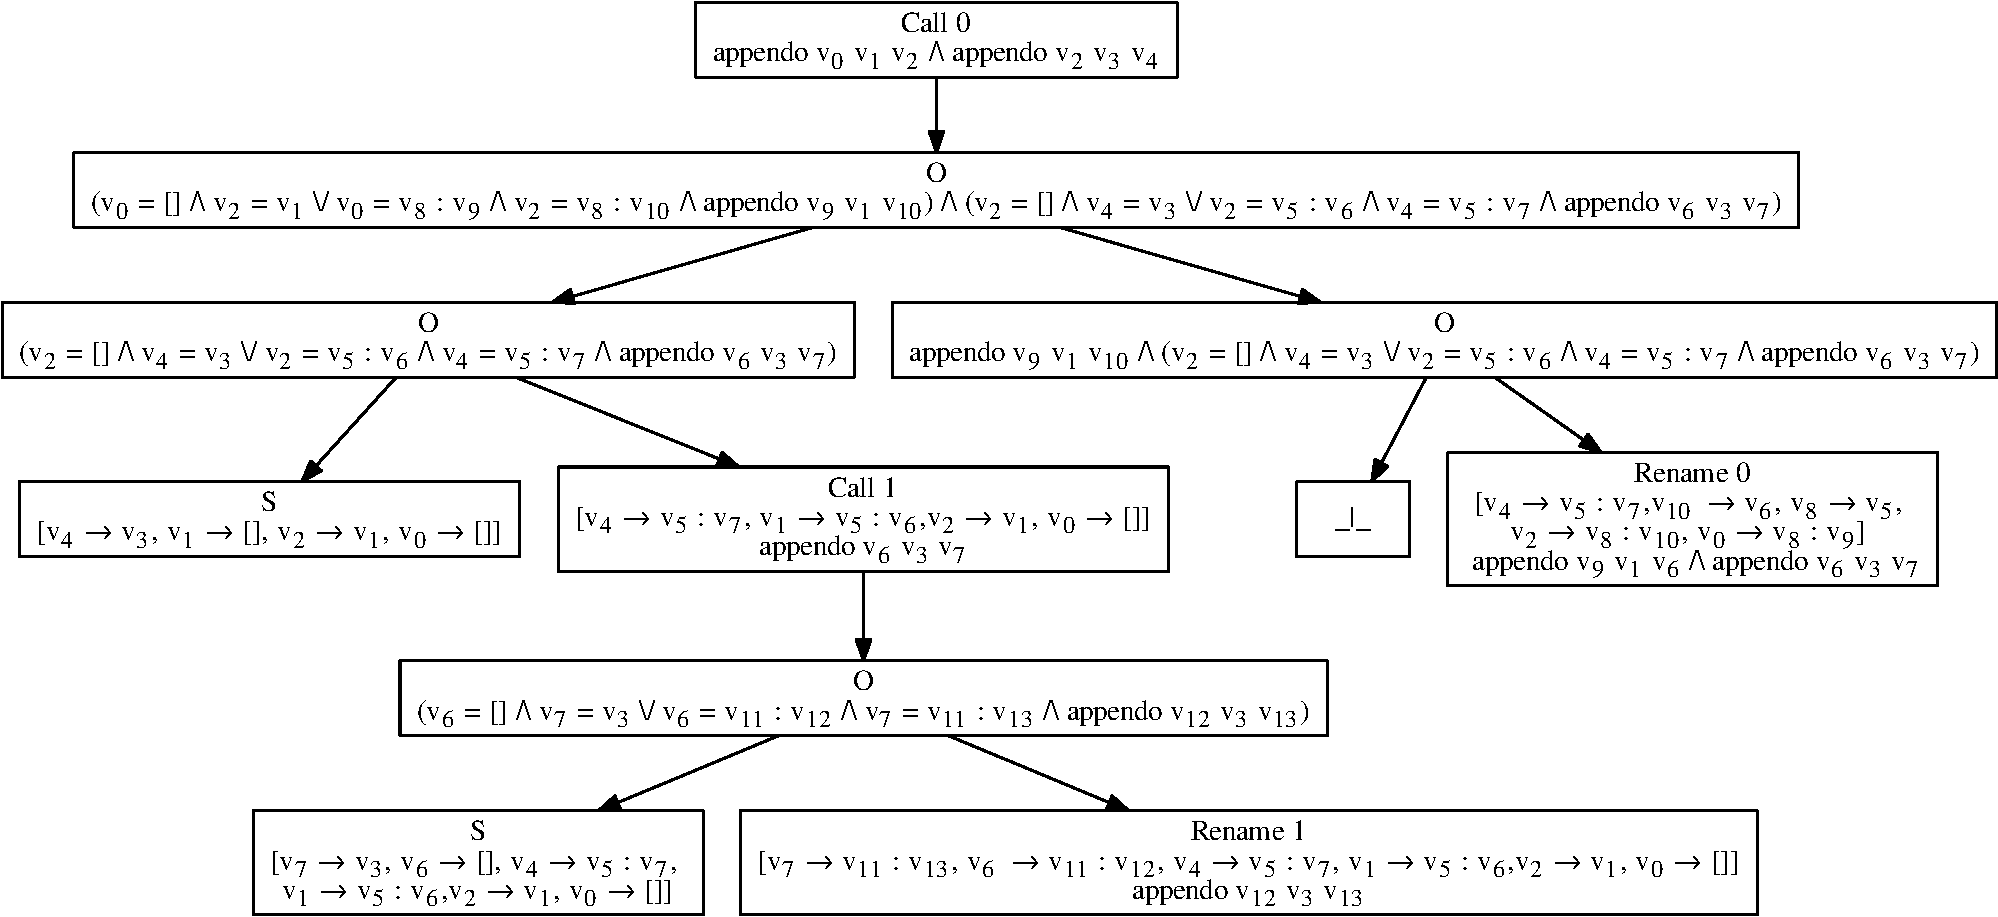
\includegraphics[width=12cm]{pics/ehm1.pdf}} 
      \end{center}
\end{frame}

\begin{frame}[fragile]
  \transwipe[direction=90]
  \frametitle{Сложности}
\begin{itemize}
  \item Что значит, что цель \emph{похожа} на другую цель?
  \item Как \emph{абстрагировать}?
  \item Как учитывается связь между переменными?
\end{itemize}
\end{frame}

\begin{frame}[fragile]
  \transwipe[direction=90]
  \frametitle{Текущее положение дел}
Реализовано несколько вариантов ``суперкомпиляции''
  \begin{itemize}  
    \item Пока все они не вполне устраивают
    \item Ищу вариант получше в литературе по частичной дедукции
  \end{itemize}
\end{frame}


\begin{frame}[fragile]
  \transwipe[direction=90]
  \frametitle{Дальнейшие планы}
\begin{itemize}
  \item Построение остаточной программы
  \item ``Негативная'' суперкомпиляция
  \item Адаптация более мощных техник символьных вычислений
\end{itemize}
\end{frame}


\end{document}